\documentclass{article}
\usepackage{geometry,framed,listings,graphicx}
\geometry{letterpaper,margin=1in}

\title{EE 445L Lab 3 Report}
\author{Firstname Lastname (eid123) \and Firstname Lastname (eid123)} \%TODO Replace everything in this field and the content between the [square brackets] with the appropriate information
\begin{document}
\maketitle

\section{Objectives}
\begin{itemize}
	\item What did you do to complete this lab? \%TODO
	\item What components were you learning about?
	\item Why do you think we made you do this lab?
	\item Aim for 5-12 bullet points
\end{itemize}

\section{Preparation Questions}

\begin{itemize}
	\item \emph{Power budget}

		def

	\item \emph{Device driver}

		def

	\item \emph{Critical section}

		def

	\item \emph{Latency}

		def

	\item \emph{Time jitter}

		def

	\item \emph{Modular programming}

		def

\end{itemize}

\section{Hardware Design}

	See the readme for info on exporting schematics.

	\includegraphics[scale=1.0]{circuit.pdf}

\section{Software Design}

	If your call graph is identical to the one in the lab document, delete this
	section. Otherwise, edit the included call graph image to accurately reflect
	your code. Make sure to export the .svg as a .pdf, as LaTeX doesn't like
	svgs.

	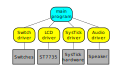
\includegraphics[scale=1.0]{callgraph.pdf}

\section{Measurement Data}
\% Note: image names and extensions should be changed to match your files

\subsection{Power noise} \% O-scope capture of the 5V and 3.3V power coming out of Launchpad
	
	\includegraphics[scale=1.0]{noise.png} 

\subsection{Speaker output} \% O-scope capture of audio signal coming out of speaker pin on Launchpad
	
	\includegraphics[scale=1.0]{speaker.png}

\subsection{Current measurements}
	
Without speaker:

With speaker on:

\section{Analysis and Discussion} \% Just gotta answer these questions

\begin{enumerate}
	\item \emph{Give two ways to remove a critical section.}

		You know the drill

	\item \emph{How long does it take to update the LCD with a new time?}

		

	\item \emph{What would be the disadvantage of updating the LCD in the background ISR?}

		

	\item \emph{Did you redraw the entire clock for each output? If so, how
		could you have redesigned the LCD update to run much faster, and create
		a lot less flicker?}

		

	\item \emph{Assuming the system were battery powered, list three ways you
		could have saved power.}

		

\end{enumerate}
\end{document}
